\documentclass[a4paper,12pt]{report}

% Paquete para inclusion de graficos.
\usepackage{graphicx}

% Paquete para definir la codificacion del conjunto de caracteres usado
% (latin1 es ISO 8859-1).
\usepackage[latin1]{inputenc}

% Paquete para definir el idioma usado.
\usepackage[spanish]{babel}


% Titulo principal del documento.
\title{TP3: Entradas de cine}

% Informacion sobre el autor.
\author{Santiago Alvarez Juli\'a, \textit{Padr\'on Nro. 99522}                     \\
            \normalsize{75.42 Taller de Programaci\'on}                             \\
            \normalsize{Facultad de Ingenier\'ia, Universidad de Buenos Aires}            \\
       }
\date{Octubre 2018}


\begin{document}

% Inserta el titulo.
\maketitle

% Quita el numero en la primer pagina.
\thispagestyle{empty}

% Crea la tabla de contenidos o indice del informe
\pagenumbering{roman}
\tableofcontents
\newpage
\pagenumbering{arabic}

% Aca arranca el cuerpo del informe
\section{Introducci\'on}

En las siguientes secciones abordar\'e algunos temas claves para la resoluci\'on del programa Entradas de cine. Estos ser\'an :

\begin{itemize}
\item Programaci\'on Orientada a Objetos (POO)
\item Protocolo de comunicaci\'on
\item Arquitectura servidor multi-cliente
\item Excepciones
\end{itemize}

\section{Temas Claves}

\subsection{Programaci\'on Orientada a Objetos}

Excepto las respectivas funciones main del cliente y el servidor, el resto del programa fue dise\~nado en base a objetos que se relacionan entre si. A continuaci\'on har\'e una breve descripci\'on de cada objeto de la aplicaci\'on.

\begin{itemize}

\item server\_Thread: este objecto encapsula la clase std::thread (que representa un hilo de ejecuci\'on). Dentro del m\'etodo start llamo al constructor de inicializaci\'on de std::thread que recibe como par\'ametros un puntero al m\'etodo run de Thread y un puntero al objecto para el cual esta definido el m\'etodo run. Dicho m\'etodo run es virtual puro, por lo tanto Thread es una clase abstracta. Esto permite que cualquier objeto pueda correr en su propio hilo mientras herede de Thread e implemente el m\'etodo run.    

\item server\_Sala y server\_Pelicula: ambos objetos contienen toda la informaci\'on de la sala y de la pel\'icula respectivamente en sus atributos. Ambos objetos solo implementan m\'etodos getters.

\item server\_Funcion: al igual que los anteriores, contiene la informaci\'on de la funci\'on en sus atributos. Adem\'as para representar los asientos de la funci\'on utilice un std::vector de std::vector de char, en el cual el primer std::vector representa la fila y el segundo la columna. Como las filas est\'an alfabetizadas, server\_Funcion tiene un m\'etodo privado llamado fila\_to\_number() que utiliza el c\'odigo ascii de los caracteres para convertir los caracteres a ints y poder acceder a una fila en el std::vector por medio de un \'indice. En este objeto se implementa la reserva de asientos y el estado de la funci\'on (si est\'a agotada o no).

\item server\_Multi\_Client\_Acceptor: es un objeto que hereda de server\_Thread, por lo que representa un hilo de ejecuci\'on y tiene su propia implementaci\'on del m\'etodo run. En detalle en la secci\'on Arquitectura servidor multi-cliente.

\item server\_ThreadServer: \'idem server\_Multi\_Client\_Acceptor. En particular se encarga de la comunicaci\'on entre el servidor y un cliente espec\'ifico mediante un common\_Socket.

\item server\_FuncionesProtected: este objecto encapsula al std::map que tiene como valores server\_Funcion y un std::map con sus respectivos mutex protectores. En detalle en la secci\'on Arquitectura servidor multi-cliente.

\item server\_main: lo primero que se hace es el parseo de los archivos de entrada. Para almacenar pel\'iculas seg\'un el genero, idioma y edad utilizo un std::vector de std::multimap (1 multimap por cada clasificaci\'on). El multimap tiene como clave un std::string y como valor un server\_Pelicula. Por lo tanto tengo cada pel\'icula en los 3 multimap, lo cual para m\'i esta bien porque pienso al servidor como una base de datos donde importa la velocidad (el m\'etodo equal\_range de multimap es O(log n)) y adem\'as se podr\'ia decir que me devuelve solo los datos que consult\'e (realmente me devuelve un par de iteradores, por lo que podr\'ia acceder a datos que no ped\'i, pero da esa sensaci\'on).

\item server\_lock: es una encapsulaci\'on RAII de la toma y la liberaci\'on del recurso mutex.

\item client\_main: parsea el std::cin para obtener las funciones que quiere ejecutar el cliente y delega la implementaci\'on de \'estas en client\_Client.

\item client\_Client: recibe los datos que vienen desde client\_main que le tiene que enviar al socket del servidor. Dependiendo de cada consulta, se llevan a cabo distintos send y receive del socket y tambi\'en se imprimen por std::cout y std::cerr algunos resultados de dicha comunicaci\'on con el servidor. 

\item common\_socket: es una encapsulaci\'on RAII del socket que implementa todas las funcionalidad necesarias (tanto para el cliente como para el servidor).

\item common\_SocketError y server\_ArchivoEntradaError: ambas son excepciones que heredan de std::exception. En detalle en la secci\'on Excepciones.

\end{itemize}

\subsection{Protocolo de comunicaci\'on}

Como los programas se comunican en su mayor\'ia enviando strings (como por ejemplo el t\'itulo de una pel\'icula), en esa mayot\'ia de casos env\'io paquetes con el formato:

|  largo  |   payload   |

Donde 'largo' es un entero de 4 Bytes en big-endian, y 'payload' es el texto a enviar, que tendr\'a el largo especificado en los Bytes que lo preceden.

Para los siguientes casos utilice otra manera de comunicarse entre el servido y el cliente, principalmente porque me parec\'ia que pod\'ia enviarse menos bits de informaci\'on de esta manera:

\begin{itemize}

\item comando del cliente: como los comando posibles son acotados, prefer\'i mandar 1 solo byte que represente a cada funcion. Por ejemplo si el cliente le env\'ia al servidor el caracter '1' al iniciar la comunicaci\'on esto significa que el cliente quiere conocer el t\'itulo de las pel\'iculas de cierto GENERO (diferentes caracteres representan distintos comandos). Para enviar al g\'enero en si (por ejemplo TERROR) utilizo el protocolo de |  largo  |   payload   |. Este protocolo es utilizado en las clases client\_Client (al comienzo de todos sus m\'etodo) y server\_ThreadServer (al comienzo de su m\'etodo run).

\item validez operaci\'on (comandos genero, idioma o edad): existe la posibilidad de que el ususarion ingrese un genero, idioma o edad inexistentes en el servidor. Por lo tanto, justo despu\'es de recibir el genero, idioma o edad en si, el servidor env\'ia un entero de 4 bytes (ahora me doy cuenta que podr\'ia ser como en el caso del comando del cliente que con 1 byte alcanza ya que hay 2 respuestas posibles) indicando la validez del comando. 

\item estado reserva asiento: (al igual que en validez operaci\'on me doy cuenta que con 1 byte alcanza ya que hay 2 respuestas posibles) el servidor para confirmar la reserva del asiento env\'ia un entero de 4 bytes que indica si la reserva fue exitosa o hubo un error (el asiento hab\'ia sido reservado anteriormente). Este protocolo es utilizado en el m\'etodo reservar\_asiento de client\_Client.

\item cantidad filas y columnas (graficar asientos): cuando el cliente le pide los datos de los asientos de una funci\'on en particular al servidor, este le env\'ia en enteros de 4 bytes la cantidad de filas y columnas que posee la sala de dicha funci\'on para facilitar el gr\'afico de los asientos. Este protocolo es utilizado en el m\'etodo asientos\_funcion de client\_Client.

\end{itemize}


\subsection{Arquitectura servidor multi-cliente}

En este programa, hay ejecuci\'on de c\'odigo en distintos hilos \'unicamente en la parte del servidor. En server\_main se lanza el hilo server\_Multi\_Client\_Acceptor cuya implementaci\'on del m\'etodo run es un while que finaliza cuando el usuario del servidor ingresa 'q' por entrada est\'andar (existe otro while, esta vez en server\_main que lee std::cin, que cuando sea el caso llama al m\'etodo stop de server\_Multi\_Client\_Acceptor). Cuando el usuario ingresa 'q', se dejan de escuchar conexiones nuevas (se cierra la conexi\'on del socket aceptador), se termina de atender a los clientes que ya están conectados, y luego se cierra la ejecuci\'on de todo el programa del servidor ordenadamente. Dentro del while de server\_Multi\_Client\_Acceptor el socket principal o aceptador acepta conexiones con nuevos clientes, una vez concretada dicha conexi\'on se lanza el hilo server\_ThreadServer que tiene como uno de sus par\'ametros el socket asociado al cliente (el devuelto por el accept del socket principal del servidor). Por lo tanto existe un std::vector de server\_ThreadServer que representan distintos clientes haciendo sus respectivas consultas al servidor.\\

Cuando es creada una instancia de server\_ThreadServer esta recibe como par\'ametros para construirse el std::vector de multimaps que contiene la informaci\'on de las pel\'iculas y una instancia de server\_FuncionesProtected. Por lo tanto ambas estructuras son recursos compartidos que deben ser protegidos cuando se utilizan hilos (del lado del servidor, std::cout y std::cerr son utilizados \'unicamente en el main thread, por lo tanto no hay que protegerlos). Adem\'as las estructuras mencionadas anteriormente deben ser tratadas de distinta manera. El std::vector de multimaps, que tienen como clave un std::string y como valor server\_Pelicula, son unicamente getters. Nunca son modificados dichos multimaps, es decir no se modifican ni las pel\'iculas internamente ni pueden ser agregadas o borradas pel\'iculas (excepto en el main thread antes de lanzar el resto de los hilos) y el m\'etodo de multimap que utilizo para recorrelo es equal\_range que por documentacion es thread safe. Por lo argumentado creo que no es necesario proteger este recurso compartido. \\

Diferente es la situaci\'on para la instancia de server\_FuncionesProtected que al contener un map donde el valor es un objeto del tipo server\_Funcion, debe ser protegida cada funci\'on por separado con un std::mutex. En este caso el std::vector de asientos es modificable durante la ejecuci\'on de hilos por lo que todos los metodos de la funci\'on que utilicen dicho atributo deben ser protegidos. En cada consulta relacionada con las funciones que el cliente tiene la posibilidad de hacer accede a los asientos, sea para saber si estan todos ocupados o para reservar un asiento. Entonces en todos los m\'etodos de server\_ThreadServer que responden a las consultas de los clientes relacionadas con las funciones son lockeados los mutex de la funci\'on espec\'ifica, permitiendo a otros hilos utilizar otras funciones.\\


\begin{figure}
\centering
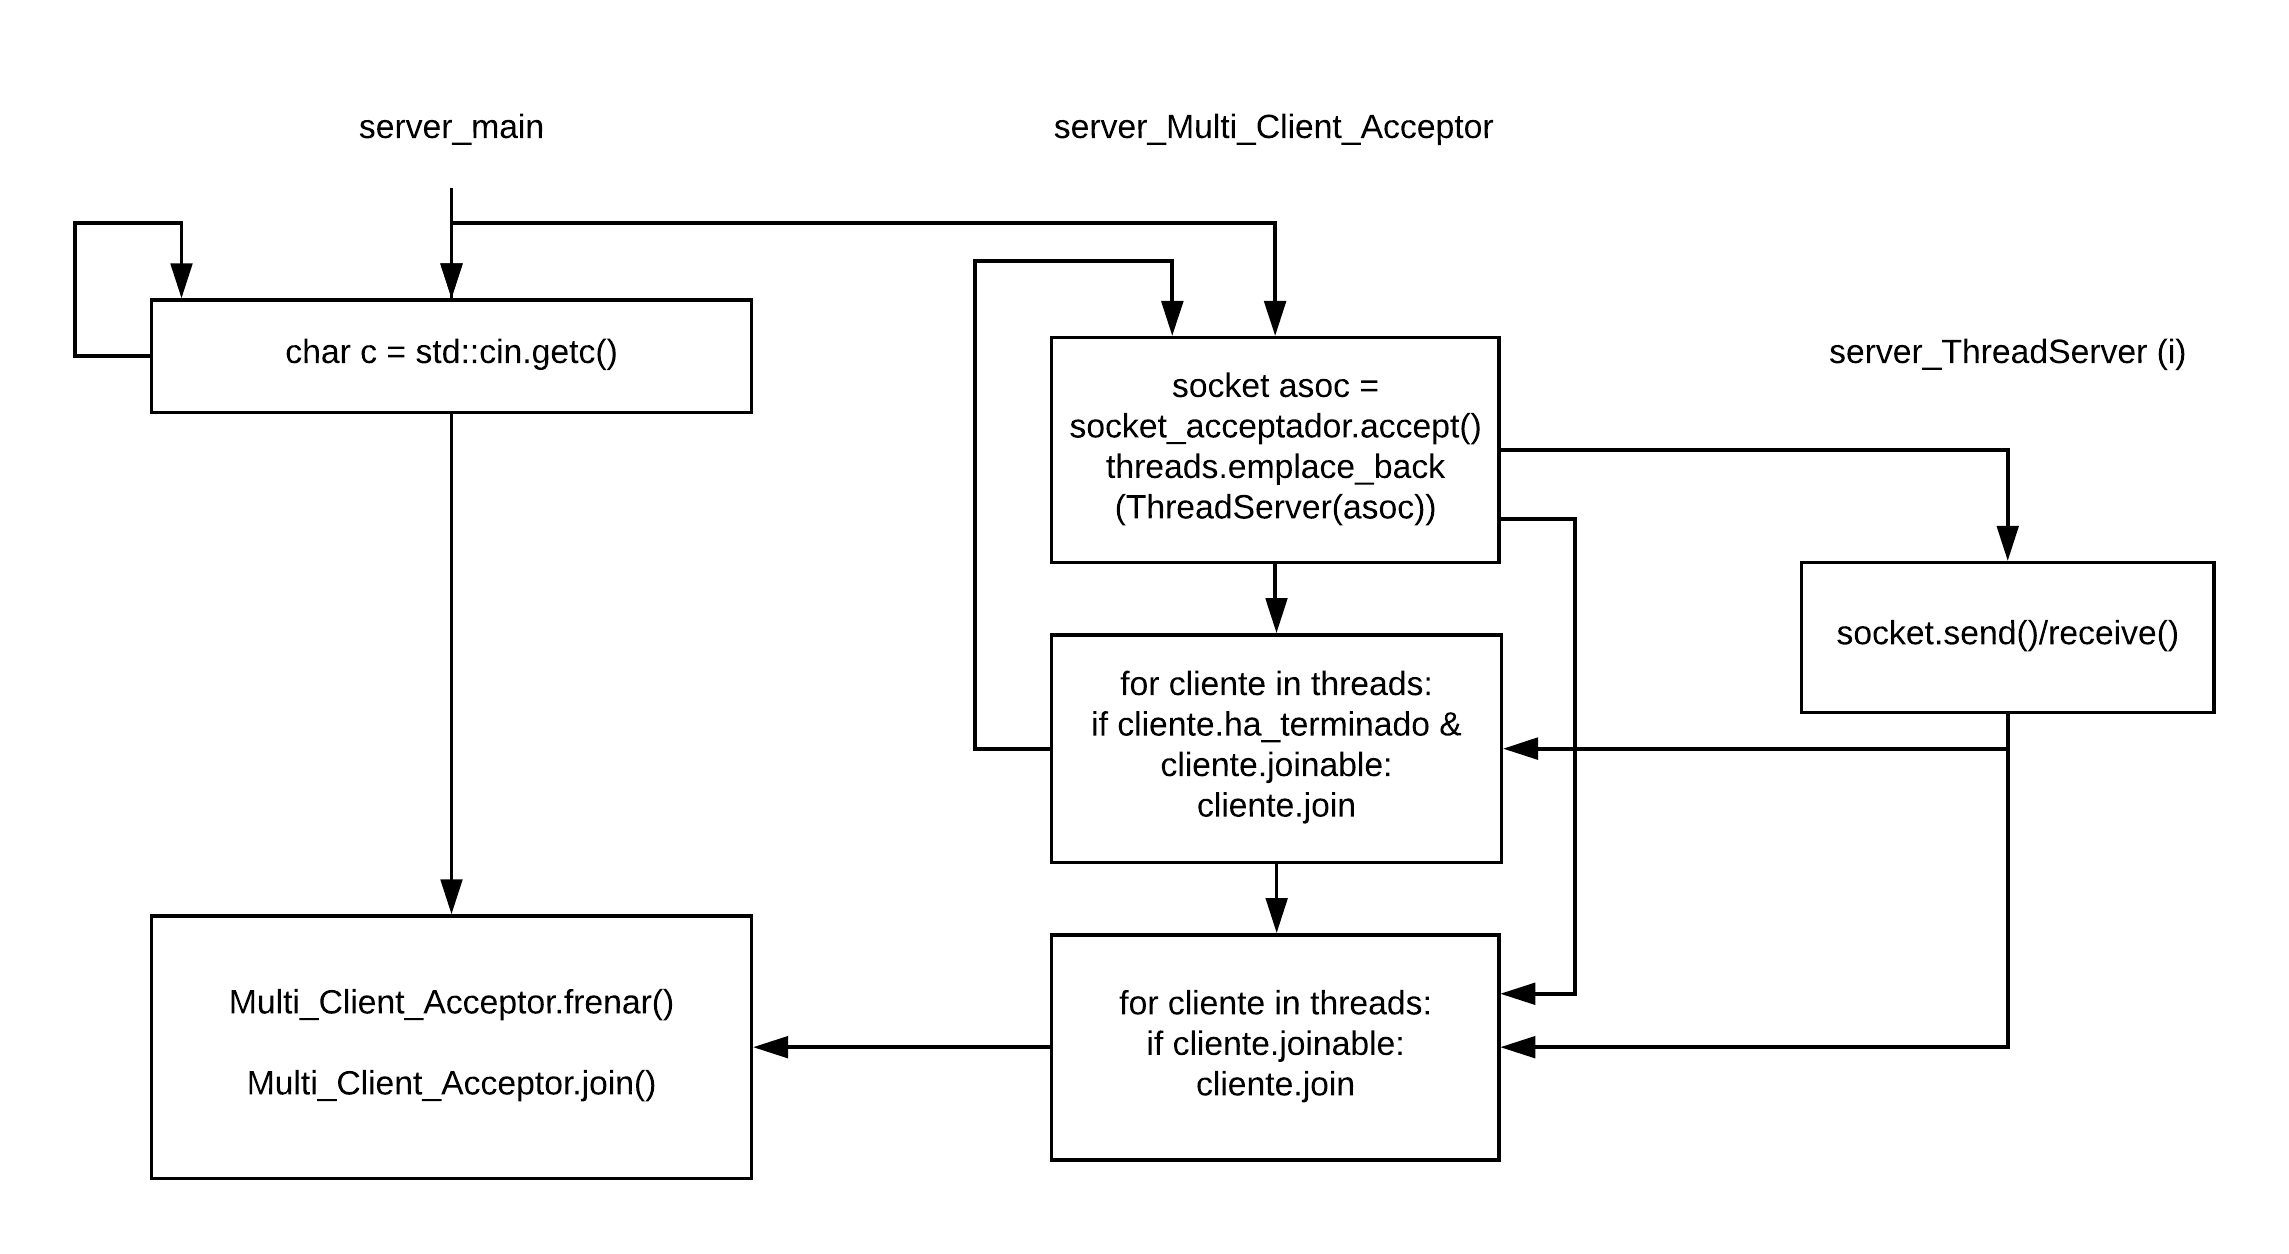
\includegraphics[scale=0.72]{servidor-multi-cliente.png}
\end{figure}


\subsection{Excepciones}

\begin{itemize}

\item server\_ArchivoEntradaError: esta excepci\'on es lanzada cuando se encuentra un error en el parseo de los archivos de entrada. Estos errores suceden cuando se hace referencia en el archivo de funciones a una sala o a una pel\'icula que no existen en sus respectivos archivos. El constructor recibe como par\'ametro un std::string que explica cual fue el error, el cual se obtiene mediante el m\'etodo what en forma de const char* y luego es impreso en std::cerr como especifica el enunciado (en el main thread del servidor).

\item common\_SocketError: esta excepci\'on es lanzada cuando se encuentra un error en el objeto common\_socket. Puede lanzarse en los siguientes metodos: constructor, connect, bind\_and\_listen y accept. Los motivos por los que suceden estos errores son diversos. El constructor recibe como par\'ametro un std::string que explica cual fue el error, el cual se obtiene mediante el m\'etodo what en forma de const char* (en este caso el error no es impreso en std::cerr, sino sería necesario proteger std::cerr ya que este error podr\'ia ser atrapado en un hilo distinto al main thread del servidor).

\end{itemize}

\end{document}